\documentclass[12pt,a4paper]{report}
\usepackage{graphicx}
\usepackage{amsmath}
\usepackage{fancyhdr}
\usepackage{cite}
\usepackage{framed}
\usepackage{a4wide}
\usepackage{float}

\usepackage{epsfig}
\usepackage{longtable}
\usepackage{enumerate}
\usepackage{afterpage}
\usepackage{multirow}
\usepackage{ragged2e}
\usepackage{gensymb}
\usepackage{amsfonts} 
\usepackage[left=1in,top=0.75in,right=1in,bottom=1in]{geometry}
\usepackage{setspace}           
\usepackage{float}
\usepackage{txfonts}
\usepackage{titlesec}
\usepackage{enumitem}
\newcommand{\Usefont}[1]{\fontfamily{#1}\selectfont}

\usepackage{lscape} % for landscape tables
\renewcommand{\baselinestretch}{1.7} 
\titleformat{\chapter}[hang]
  {\normalfont\LARGE\bfseries}
   {\thechapter.}
  {0.01em}
  {}
\titlespacing*{\chapter}{0pt}{*3}{*2}

\usepackage{blindtext}
\usepackage{xpatch}
\usepackage{url}
\usepackage{leqno}
\usepackage{subcaption}
\linespread{1.5}
\usepackage[intoc, english]{nomencl}
\hyphenpenalty=5000
\tolerance=1000
\usepackage[nottoc]{tocbibind}
\setlength{\parskip}{1em}
% ******* References config *********
\bibliographystyle{IEEEtran}   % On some TeX systems this works
%\bibliographystyle{ieeetr}      % While on others this works
							% Uncomment and test if your references don't cite
							% correctly
\renewcommand{\bibname}{References}

\title{GPCPKS SeminarReportTemplate}
\author{sudevank }
\date{July 2024}

\begin{document}
\gdef \title{How to prepare a Seminar report using \LaTeX } % Seminar title
\gdef \author{Student Name}	 %student name
\gdef \dept{Electronics  Engineering} %Department
\gdef \degree{Diploma } %degree
\gdef \branch{Electronics  Engineering} %branch
\gdef \college{Government Polytechnic College}
\gdef \collegeplace{Palakkad}
\gdef \rollno{TVE17EC0XY} %KTU Reg No
\gdef \deptabbr{Dept.of Electronics} %Dept name abbreviation
\gdef \guide{Lecture-1}
\gdef \hod{Dr. Dileep P} %Head of Department
\gdef \hoddes{Professor and Head} %HOD designation

\gdef \acadyear{2024 - 25} % Academic year
\gdef \month{November 2024} %Month of Report submission
\gdef \date{21-11-2020} %Date of signing the declaration
\setcounter{secnumdepth}{1} 

\newenvironment{coverpage}
\thispagestyle{empty}
\begin{titlepage}
 
  \noindent%
  
  \begin{center}
  	
\includegraphics[width=50mm]{figures/tu.jpg}\\
  
\textsc{\LARGE \bfseries TRIBHUVAN UNIVERSITY}\\[0.5cm] % Name of your university/college
\textsc{\large \bfseries INSTITUTE OF ENGINEERING}\\
\large \textbf{ Paschimanchal Campus } \\[0.5cm]
\vspace{0.5cm}
\Large \textbf{Ice-Cream Production Plant}\\[0.5cm]
%\large \textbf{Subject code} \\[0.2cm]
\vspace{0.5cm}
\textbf{By:}\\
\large{ Sworup Bhandari   (PAS078BCT046) \\
Seamoon Pandey()\\
Nisha Pandey()\\
Smriti Rana()}\\
\vspace{1.2cm}
A PROJECT PROPOSAL TO THE DEPARTMENT OF ELECTRONICS AND COMPUTER
	ENGINEERING IN PARTIAL FULFILLMENT OF THE REQUIREMENT FOR THE BACHELOR'S
	DEGREE IN Computer ENGINEERING \\[1.2cm]


\textbf{Department of Electronics and Computer Engineering}\\
Pokhara, Nepal
\\[0.4cm]
\vspace{0.5cm}

\end{center}
\end{titlepage}

\pagenumbering{roman} 
%%==================================acknowledgement.tex=============================
\chapter*{Acknowledgement}%
\addcontentsline{toc}{chapter}{Acknowledgement}%

%\newenvironment{acknowledgement}


I take this opportunity to express my deepest sense of gratitude and sincere thanks to everyone who helped me to complete this work successfully. I express my sincere thanks to \textbf{ \hod}, Head of Department, \dept, \college\hspace*{2pt} \collegeplace \hspace*{2pt} for providing  me with all the necessary facilities and support.\par

 I would like to express my sincere gratitude to \textbf{\guide}, \hspace*{2pt} department of \hspace*{2pt} \dept, \hspace*{2pt} \college \hspace*{2pt} \collegeplace \hspace*{2pt} for their support and co-operation.


Finally, I thank my family, and friends who contributed to the successful fulfilment of this seminar work.

\vspace*{30pt}
\begin{flushright}
	\textbf{\author}
\end{flushright}
\thispagestyle{plain}

%============================= abstract.tex================================
\chapter*{Abstract}%
%\addcontentsline{toc}{chapter}{\numberline{}Abstract}%
\addcontentsline{toc}{chapter}{Abstract}%
Travel Buddy is a cutting-edge web app created to improve the trip by resolving typical issues encountered by tourists. The web app provides a customized travel experience, makes travel planning easier, and links users with like-minded people. Finding travel partners based on common interests, suggesting off-the-beaten-path locations, and enabling smooth communication are important elements. To assist users with travel budgeting, the app also incorporates an expense management function. Travel Buddy makes travel more pleasurable by combining logistics, social connectivity, and itinerary preparation. According to a study with fifty respondents, there was a great deal of interest in a platform that dealt with travel and friendship.



\section*{Keywords}

Mobile App, Travel Planning, Companions, Personalized Experience, Itinerary Management, Expense Tracking, Recommendation System, User Engagement


\thispagestyle{plain}
%=======================================================================

 



\thispagestyle{empty}
\newpage
\tableofcontents
\listoffigures
%\listoftables

\cleardoublepage
\setcounter{page}{1}
\pagenumbering{arabic}
\chapter{ Introduction}
With so many new places to discover and memories to create, traveling is a thrilling journey. However, there are challenges as well, such as organizing travel, handling finances,locating undiscovered places to go and the hardest, finding the right person to share the trip with. 

The nicest part of any trip is sharing it with someone. For this reason, we developed Travel Buddy, not just an app but an experience that not only assists with trip planning and organization but also serves as a platform for connecting with like-minded travelers.

\textbf{\textit{Who do I visit my dream place with? Well, the travel agent might plan it, but the travel buddy makes it unforgettable, because every journey needs a copilot for snacks and selfies!}}

Every trip is made more enjoyable and unforgettable with Travel Buddy, whether it is for friendship, adventure, or simply enjoying each other's company.

\chapter{Objective}

Travel Buddy seeks to improve passengers' entire experience by addressing the typical problems they encounter. The application's goals are to make travel planning easier, create deep connections, and offer resources for a more pleasurable and hassle-free experience. The following are Travel Buddy's main goals:
  \begin{enumerate}
    \item Connect Travelers: Create a platform for users to find like-minded travel companions based on shared interests, destinations, or travel styles.
    \item Discover Hidden Gems: Recommend off-the-beaten-path attractions and experiences tailored to user preferences.
    \item Connection: Enable users to communicate with one another, share plans, and organize trips together seamlessly.
    \item Manage Finances: Include an integrated expense management feature to help users track and budget their travel costs.
\end{enumerate}

\pagebreak
\chapter{Literature Review}
Travel Buddy, a travel application for itinerary planning and finding companions, builds upon existing research in tourism systems. The following literature review highlights key studies and platforms that influence its development.

\section{ Tourism Websites and Creative Itineraries}
Traditional travel websites often provide broad information but lack creativity in itinerary planning. A study in the International Journal of Scientific Research in Engineering and Management (2023) proposes a system for generating creative travel plans through information abstraction, reuse, and formulation. By ranking itineraries based on creativity, this system personalizes travel planning, which aligns with Travel Buddy’s goal of customized travel plans \cite{ijsrem2023}.

\section{ Smart Tourism Systems}
Al Saeed et al. (2020) address the need for smart tourism systems that cater to diverse tourist values like emotional and social experiences. Their "Travel Key" application, which provides personalized recommendations based on user preferences, serves as a model for Travel Buddy. It leverages user data to match travelers with compatible companions and enhance the overall experience \cite{alsaed2020}.

\section{ Existing Travel Platforms}
Platforms such as Be a Travel Buddy, Workaway, and TripGiraffe focus on connecting travelers with similar interests. These platforms highlight the growing demand for social travel experiences, which Travel Buddy integrates by allowing users to find travel companions while also managing logistics and itineraries\cite{beatravelbuddy}\cite{workaway}\cite{tripgiraffe}.

\section{Challenges in Comprehensive Applications}
Many travel apps focus on individual aspects like booking or itinerary planning but lack integration. Travel Buddy aims to unify these features, incorporating recommendation algorithms and creative itinerary generation to offer a more holistic travel experience.


The reviewed literature demonstrates the need for an integrated platform like Travel Buddy, which combines itinerary planning, travel logistics, and social connectivity. This comprehensive approach meets the evolving demands of modern tourists.

\chapter{Project Feasibility  and Statistics}
By bringing like-minded travelers together, streamlining trip planning, and providing tailored recommendations, the Travel Buddy app is a creative way to improve the travel experience. To ascertain the Travel Buddy project's viability and commercial potential, this feasibility study assesses its technical, operational, social, legal and financial viability.
\section{Market Viability}
\begin{enumerate}
  
 \item Target Market: Young adults, frequent travelers, and lone travelers looking for company and individualized travel experiences make up Travel Buddy's main target market. There is a significant market need, as seen by the growing popularity of social travel and the rising use of smartphone apps for trip planning.

 \item Competitive Analysis: While some travel applications now on the market concentrate on specific areas, such reservations or itineraries, very few incorporate social media and provide all-inclusive solutions. By fusing social networking, expenditure management, and trip planning, Travel Buddy distinguishes itself in the industry.

 \item Market Demand: According to a study of 71 participants, a sizable portion of them indicated interest in using a platform to arrange travel plans and discover travel companions. This validates the demand for such an app and supports the market potential.
\end{enumerate}
\section{Regulatory and Legal Viability}
\begin{enumerate}

    \item Data Privacy: It's critical to protect user privacy and data. To protect user data, the app will abide by GDPR rules and other applicable data protection laws. Secure payment gateways will be incorporated for in-app purchases, and a transparent privacy policy will be written.

    \item Intellectual Property: The user interface design and recommendation engine, among other distinctive features of Travel Buddy, will be safeguarded by intellectual property rights. Additionally, efforts will be made to register the app's name and logo as trademarks.

\end{enumerate}
\section{}
\begin{enumerate}

    \item User Experience: The success of the app will largely depend on the design of the user interface (UI) and user experience (UX). Engaging users and motivating them to use the app frequently depend on a straightforward, user-friendly design. Frequent user testing will be part of the operational process to make sure the app stays user-friendly.

    \item Customer Support: To address questions, comments, and problem solving, an effective customer support system will be incorporated into the app. For routine questions, this can be accomplished via a chatbot; for more complicated problems, a ticket-based system can be used.

    \item Collaborations and Partnerships: By providing users with special offers and discounts, forming alliances with travel agencies, transit companies, and lodging providers can improve the app's value proposition.
 
\end{enumerate}
\chapter{Requirements}
\section{Functional requirements}
\begin{enumerate}
    \item Authentication: 
    \begin{itemize}
        \item The user shall be able to sign in with credentials and generate a authenticated session for the user. 
        \item The user shall be able to register with an account with minimal input taken.
    \end{itemize}

    \item User profile:
    \begin{itemize}
        \item The user shall have two status ie: (verified and unverified), with verified being adding the id's and others being unverified.
        \item The user shall be shown an onboarding page with their incomplete data status.
        \item The verified user can view the status of other user but and uverified user can't view the status of the other user.
        \item The user should be able to add their hobbies and interests.
    \end{itemize}

    \item Post: The user should be allowed to post their images featuring some destinations or places of interests.
    \item Suggestions:
    \begin{itemize}
        \item The application shall suggest user friends and connections according to their hobbies and their profile verification status.
        \item The application shall suggest the user some places to visit according to the rating and preferences of people with similar interests.
        \item The application shall provide a place to reach out with like minded individuals who want to travel together or are unable to go on a trip due to lack of company.
        \item The application shall implement some strict rules and regulations to regulate the misuse of the platform.
    \end{itemize}

    \item Ratings:
    \begin{itemize}
        \item The platform should have rating system for ranking the suggestions.
        \item The users should be able to rate each other once they plan a trip in the application for the authenticity of the users.
    \end{itemize}

    \item Connection:
    \begin{itemize}
        \item The user should have the ability to establish connection with another user just like social media applications with accepting and rejecting features.
        \item Connected users shall be able to chat with each others.
        \item Chat shall be in real time.
        \item Users shall be able to form groups.
    \end{itemize}
    \item Plans: User shall be able to create plans and the user with common plans and same verification level shall be suggested to each other.
\end{enumerate}


\section{Non-Functional requirements}
\begin{enumerate}
    \item Usability: The platform should have an intuitive and user-friendly interface, which is easy to access and use.
    \item Performance: The platform should load within 2 seconds for standard broadband connections.
    \item Scalability: The platform shall support a minimum of 1000 users initially, with room for scaling up.
    \item Security: It should have a secure user authentication (e.g., HTTPS, encrypted passwords).
    \item Maintainability: The code base should be modular and follow standard coding guidelines so that the code can be maintained and updated routinely.
    \item Localization: The app should support time, date, and currency format according to user settings.
    \item Consent: The users shall be explicitly notified about the code of conduct in the terms and conditions consent agreement.
\end{enumerate}

\chapter{Diagrams}

\section{Dataflow diagram}
\begin{figure}
    \centering
    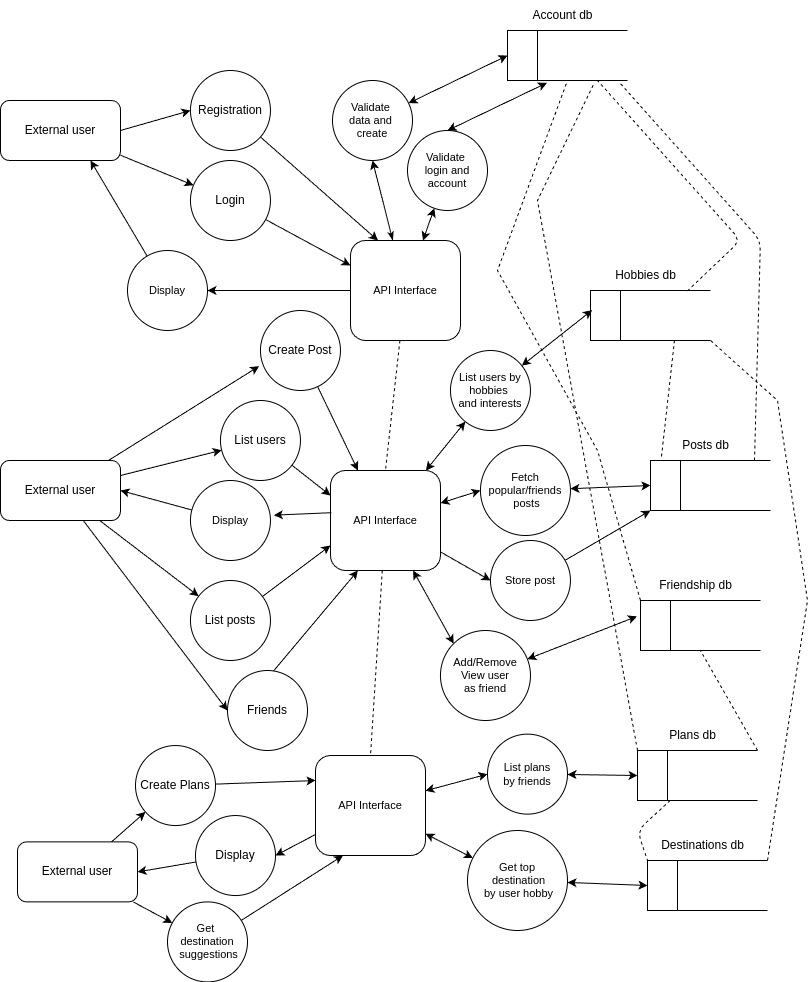
\includegraphics[width=\textwidth, keepaspectratio]{figures/dataflow.png}
    \caption{Dataflow Diagram for Travel Buddy}
    \label{fig:dataflow}
\end{figure}




\chapter{Conclusion}

\raggedright
\bibliography{refs}	
\end{document}
